% KFRA composition before

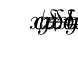
\begin{tikzpicture}
    % first layers
    \node (in1)
        [inner sep=0]
        {\tikz \drawMessagesWithArrows{$x$}{$\delta x$}{$\HeCal  x$}{\hNodeDistance};};
    \node (activation)
        [anchor=south west, inner sep=0]
        at (in1.south east)
        {\tikz\drawModuleNoParams{$\phi$}{5};}; 
    \node (out)
        [inner sep=0, anchor=south west]
        at (activation.south east)
        {\tikz \drawMessagesWithArrows{$y$}{$\delta y$}{$\HeCal  y$}{\hNodeDistance};};      
    \node (layer1)
        [anchor=south west, inner sep=0]
         at (out.south east)
         {\tikz \drawModuleWithParams{$z = Wy$}{16}{\hspace{1.5ex}$ W$\hspace{1.5ex} }{\,$\delta  W$\,\,}{$\HeCal W$};};
    \node (layer2)
        [inner sep=0pt, anchor=south west]
        at (layer1.south east)
        {\tikz\drawModuleWithParams{$+ b$}{16}{$b$}{$\delta b$}{$\HeCal  b$};};
    \node (out2)
        [inner sep=0, anchor=south west]
        at (layer2.south east)
        {\tikz \drawMessagesWithArrows{$z$}{$\delta z$}{$\HeCal  z$}{\hNodeDistance};};       
\end{tikzpicture}	